\documentclass{article}
\usepackage{inputenc,amsmath,upquote,amssymb}
\usepackage{graphicx}
\usepackage[hyphens]{url}
\usepackage[margin=1.40in]{geometry}
\usepackage[style=authoryear,maxbibnames=9,maxcitenames=1,backend=biber]{biblatex}
%\usepackage[]{natbib}
\usepackage[toc,page]{appendix}
\addbibresource{bibliography.bib}

\begin{document}
\title{Distributed Representation of Sentences for Speculative Language Recognition in Biomedical Articles}
\author{Jia-Shen Boon \and Rasiga Gowrisankar \and Akshay Sood}
\date{Fall 2014}
\maketitle

\begin{abstract}


We explore the automatic identification of speculative language in biomedical articles using distributed representation of sentences and deep learning methods. Such an identification has potential applications in information retrieval, multi-document summarization and knowledge discovery. We explore two methods that learn distributed representations of sentences, Paragraph Vector model and Recursive Neural Tensor Network, and compare them against  three baseline algorithms, Support Vector Machines, Naive Bayes and pattern matching. We show that the RNTN (F1 = 0.885) marginally outperforms the best baseline algorithm, linear bigram SVM (F1 = 0.881), while the paragraph vector approach performs poorly (F1 = 0.368) even after training with a large unlabeled dataset. We discuss reasons for these differences in performance and give suggestions for future work.
% * <jiashen@gmail.com> 2014-12-17T19:28:10.109Z:
%
%  we'll need to update this when we get the curves. My impression is that RNTN outperforms our best baseline algorithm but the paragraph vector approach performs significantly worse than both RNTN and SVM, even when trained with a large unlabeled dataset.
%
% ^ <rasiga.g@gmail.com> 2014-12-18T02:31:33.848Z.


\end{abstract}

\section{Introduction}

	Published articles in the biomedical field include both established solid facts and new emerging less solid knowledge that represents new thoughts or findings \autocite{Medlock2008}. Consider the following example sentences:

{\it The study proves that the promoter is effective.}

{\it The study suggests that the promoter may be effective.}

The second sentence includes cue words and phrases such as {\it suggests that} and {\it may be} which render the scope, {\it the promoter is effective} to be speculative. Automatic recognition of such speculative statements would ensure that an Information Retrieval system does not misrepresent less solid information as being facts. Prior work in this domain has been carried out using pattern matching \autocite{Malhotra2013}, probabilistic weakly supervised learning models and Support Vector Machines \autocite{Medlock2007}. All of these methods use the bag-of-words approach for representing the text, where each element indicates the presence or frequency of a word (for unigram BoW) or a pair of words (for bigram BoW). The bag-of-words approach has two major weaknesses: it loses the ordering of the words and also ignores the semantics of the words \autocite{Le2014}. The ordering and semantics of the words are important for the speculative language recognition task as the speculativeness of a sentence depends not just on the presence of cue words but also on the context in which they appear.

It has been shown that a distributed representation of words can capture semantic information \autocite{mikolov2013efficient}. This is a representation with continuous rather than Boolean or integer features as is the case for BoW. Recent advances in machine learning have made possible the learning of distributed representations of not just words, but sentences and text of arbitrary length as well. In this study, we explore the possibility of using distributed representation of sentences using two approaches: Paragraph Vectors \autocite{Le2014} and Recursive Neural Tensor Network \autocite{Socher2013}. We hypothesize that applying distributed representation of sentences to the task of speculative language recognition in biomedical articles improves the performance in the task, compared to baseline algorithms. The performance of these two methods and that of the baselines is evaluated using their F1 scores, ROC curves and Precision-Recall curves.

The subsequent sections are organized as follows: related work is presented in Section 2. Section 3 describes in detail the Paragraph Vector representation and Recursive Neural Tensor Network methods. The evaluation of these methods against the baselines considered is presented in Section 4. Section 5 consists of discussions, findings, limitations of the approaches used and future work. We conclude in Section 6.

Our code is available online.\footnote{
\url{https://github.com/boonjiashen/speculative-language-recognizer}}

\section{Related work}
The task of speculative language recognition, especially in the biomedical domain, has been researched upon for many years. An SVM-based text classification approach and a substring matching approach are discussed in one of the earliest papers addressing this task \autocite{Light2004}. In \textcite{Medlock2007}, a weakly supervised probabilistic model for training data acquisition and classification is proposed. Their model is based on Naive Bayes with smoothing to avoid unreliable frequency estimates when the amount of training data is limited. We explore a similar approach as one of our baselines. A Bayesian logistic regression classifier using a Laplace prior is proposed in \textcite{vlachos2010detecting}. They approach speculation detection as a token classification task where each token is identified to be a cue or not. They also determine the scope of each cue word. A more recent work described in \textcite{Malhotra2013} is a pattern matching approach using a dictionary of speculative patterns. 


\section{Methodology}

\subsection{Datasets}
Our labeled dataset comes from the BioScope corpus \autocite{bioscope}; our unlabeled dataset comes from BioMed Central \autocite{biomed}. The BioScope corpus is a dataset of biomedical articles described in XML. Each sentence is parsed as follows. For each speculative sentence, the cue word/phrase that causes the speculation is tagged, as well as the scope of speculation. In the following illustrative example,

\begin{verbatim}
<sentence> 
    The novel enhancer element identified in this study is 
    <xcope> 
        <cue type="speculation">probably</cue> 
        a target site for both positive and negative factors.
    </xcope>
</sentence>
\end{verbatim}

The scope of the entire sentence is demarcated, the speculative cue word {\it probably} has been tagged, and the scope of speculation {\it probably a target site for both positive and negative factors} has been tagged as well.

The BioMed corpus also comprises biomedical articles in XML. It differs from the BioScope corpus in two key aspects. It is much larger (over 200000 articles as compared to 1273 abstracts and 9 full papers in the BioScope corpus), and sentences are not labeled speculative/non-speculative. We use a subset of the BioMed corpus to augment the training set of the Paragraph Vector approach. All other approaches are trained and tested on the BioScope corpus only.

All sentences in the dataset are converted to lower-case.
% * <rasiga.g@gmail.com> 2014-12-17T19:06:31.887Z:
%
%  add BioMed citation
%

\subsection{Paragraph vector representation}

The paragraph vector (PV) approach follows that described in \textcite{Le2014}. It comprises two models. At test time, the paragraph vector model outputs a fixed length vector for the test sentence. Then a logistic classifier outputs a binary label given the paragraph vector.\footnote{To remain consistent with the terms used in \textcite{Le2014}, we use the term `paragraph vector' to refer to the fixed length feature vector of a sentence. In this study, test and training instances are sentences, but the paragraph vector algorithm is able to learn feature vectors for text of arbitrary length (e.g., phrases, sentences and paragraphs).}

\paragraph{Dataset} The dataset is partitioned as follows. We assign 70\% of the sentences of the BioScope corpus to the training set and 30\% to the test set. To exploit a large unlabeled dataset, we append sentences from a subset of the BioMed corpus to the training set, if applicable. As such, the PV model is trained on a mixture of labeled and unlabeled sentences.

\begin{figure}
\centering
    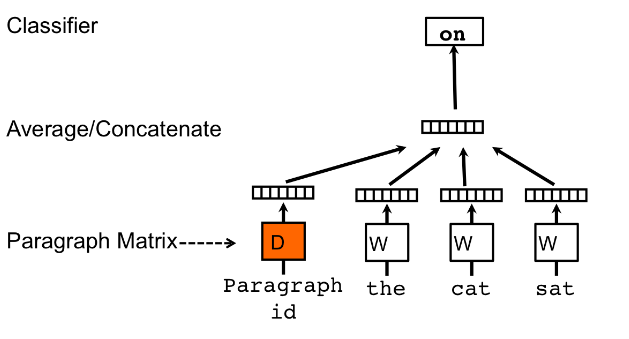
\includegraphics[width=0.65\textwidth]{PVexample.PNG}
\caption{Network architecture of the Paragraph vector model \autocite{Le2014}}
\label{fig:PV}
\end{figure}
\paragraph{Training the PV model} The architecture of the PV model is shown in Figure~\ref{fig:PV}. It is known as the Distributed Memory Model of Paragraph Vectors. The model maintains a word vector matrix $W \in \mathbb{R}^{N \times p}$ and a paragraph vector $P \in \mathbb{R}^{M \times p}$, where $N$ is the number of training sentences, $M$ is the number of unique words in the training set, and $p$ is the length of one feature vector. The input layer is a concatenation of the paragraph vector of the training sentence and the word vectors of the words in a sliding window over the training sentence. The output layer is a softmax layer. The training objective is to predict the next word after the sliding window. This objective function is minimized via stochastic gradient descent where the gradient is computed via backpropagation. The error gradients are backpropagated up to and including the input layer.

At training time, we learn $W$, $P$ and the softmax weights. We use the F1 score of a logistic classifier to evaluate the quality of the PV model and to decide when to stop training.\footnote{We do this instead of monitoring the training error due to a limitation in the \texttt{gensim} library. The API does not return the training error after each epoch.} After every training epoch, we learn a logistic classifier with the learned paragraph vectors that have labels. These are the sentences from the BioScope corpus. We stop training the PV model when the F1 score of this logistic classifier starts to drop, i.e., just after the F1 score is maximized. See the discussion section for other evaluation methods that have been considered. The learning rate is constant at 0.001 while the feature length $p$ is 52. No cross-validation is performed.

\paragraph{Training the logistic classifier} After the PV model has been trained, we train the second model of the PV approach, which is a logistic classifier. The training examples are the learned paragraph vectors from the BioScope corpus and their corresponding labels. In practice, we just take the logistic classifier last trained during the training process of the PV model (see above).
% The task of the first network is to learn the fixed length feature vector of a test sentence. This network uses the Paragraph Vector algorithm where every word and every sentence is mapped to a unique vector. The paragraph vector and the word vectors are concatenated or averaged to predict the next word in the sentence. The paragraph vector remembers what is missing from the current context. The contexts are fixed-length and sampled from a sliding window (we use a wondow of length 3) over the sentence. Thus word vectors, paragraph vectors and softmax weights are learnt for all sentences in the training set. This training phase is unsupervised and uses unlabeled data.

%\paragraph{Training the logistic classifier} The second network is a logistic classifier that takes the paragraph vector for each sentence produced by the first network as input to predict whether that sentence contains speculative language. By inputing the training instances, the network parameters such as ..... are learnt using stochastic gradient descent.

\paragraph{Testing a new sentence} At test time, we freeze the softmax weights and $W$, and run a sliding window over the test sentence to learn a paragraph vector by stochastic gradient descent. This paragraph vector is then labeled by the logistic classifier. The number of epochs at test time is held constant at 50 and the learning rate is 0.001.
% * <rasiga.g@gmail.com> 2014-12-17T18:35:45.583Z:
%
%  mention the network parameters trained
%
% ^ <jiashen@gmail.com> 2014-12-18T04:54:19.663Z.

\paragraph{Implementation details} The PV model approach was implemented in Python. We use the \texttt{gensim} library for the PV model and the \texttt{scikit-learn} library for the logistic classifier. To split a textblock from the BioMed corpus to a list of sentences, we use the NLTK English Punkt Sentence Tokenizer. To split a sentence into a list of words/punctuation, we use NLTK's \texttt{nltk.word\_tokenize} function.

\begin{figure}
\centering
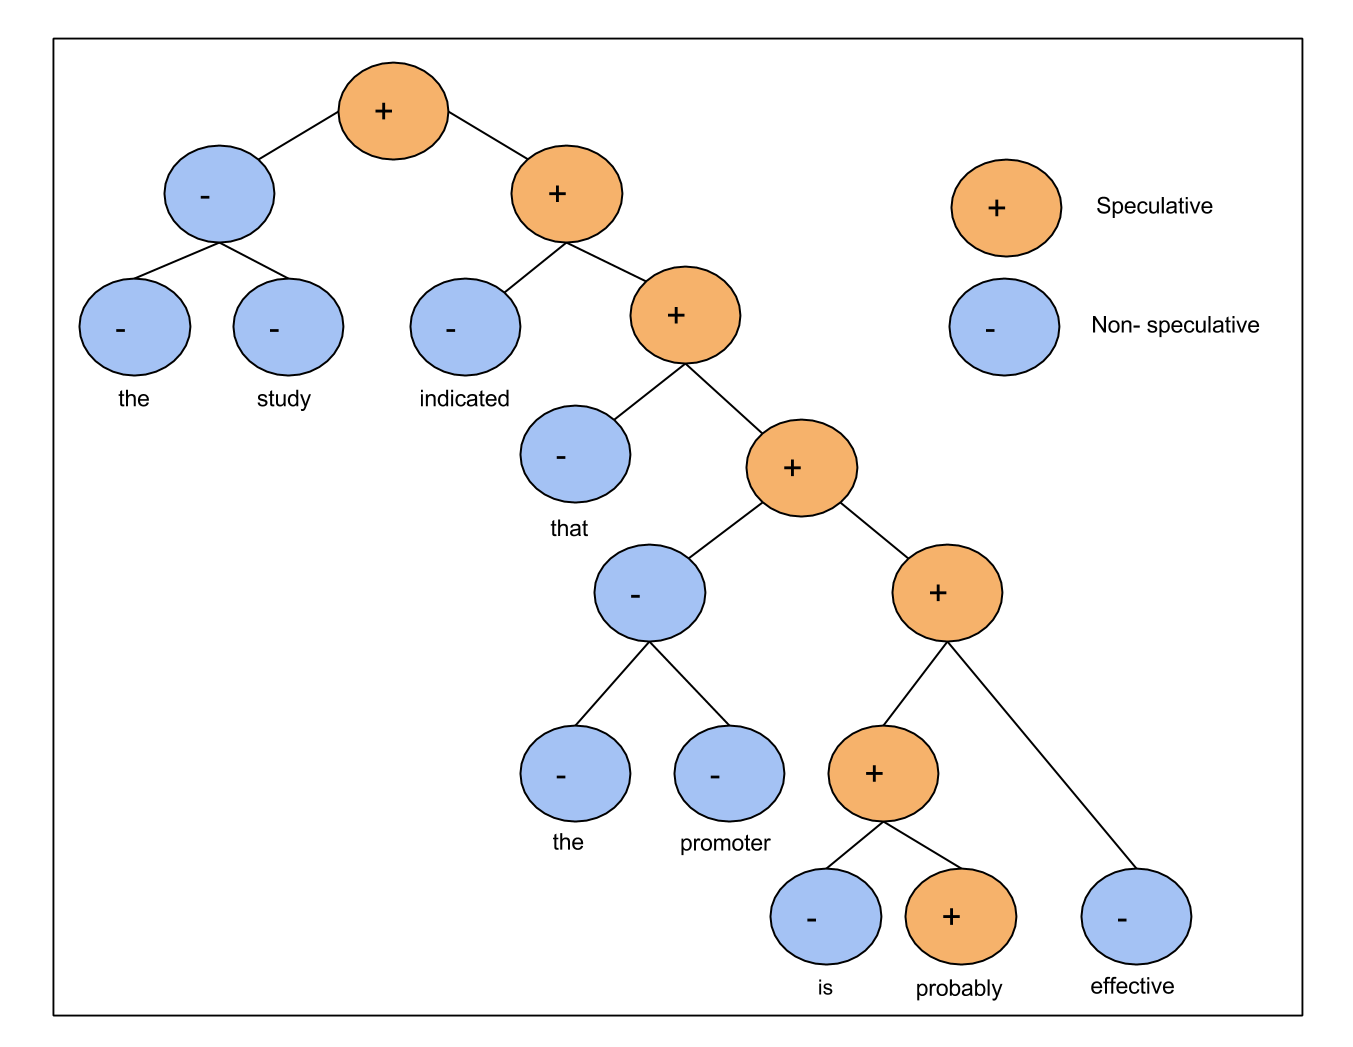
\includegraphics[width=6.5cm,height=8.2cm,keepaspectratio]{SpecParseTree.png}
\caption{Speculation labeled parse tree for the example sentence {\it the study indicated that the promoter is probably effective}}
\label{fig:parsetree}
\end{figure}

\subsection{Recursive Neural Tensor Networks}

A semantic vector space for single words does not capture the meaning of longer phrases properly. To remedy this, \textcite{Socher2013} propose the use of a fully labeled parse tree to analyze the compositionality of sentiment in language. The Stanford Sentiment Treebank used in this paper consists of binary parse trees generated by the Stanford parser and manually annotated by human judges. To capture the compositional effects with higher accuracy, \textcite{Socher2013} proposed the Recursive Neural Tensor Network (RNTN). RNTNs take as input phrases of any length. These networks represent a phrase through word vectors and a parse tree and then compute vectors for higher nodes in the tree using the same tensor-based composition function. We explore the possibility of applying the same idea to the task of speculative language recognition.  Since our data set - the BioScope corpus \autocite{Vincze2008} has the speculative cue words tagged, we use it for annotating our parse trees instead of human judges.

We now describe the generation and labeling of parse trees and training the RNTN with an example sentence: {\it``the study indicated that the promoter is probably effective''}.

\begin{figure}
\centering
\begin{minipage}{.45\textwidth}
\centering
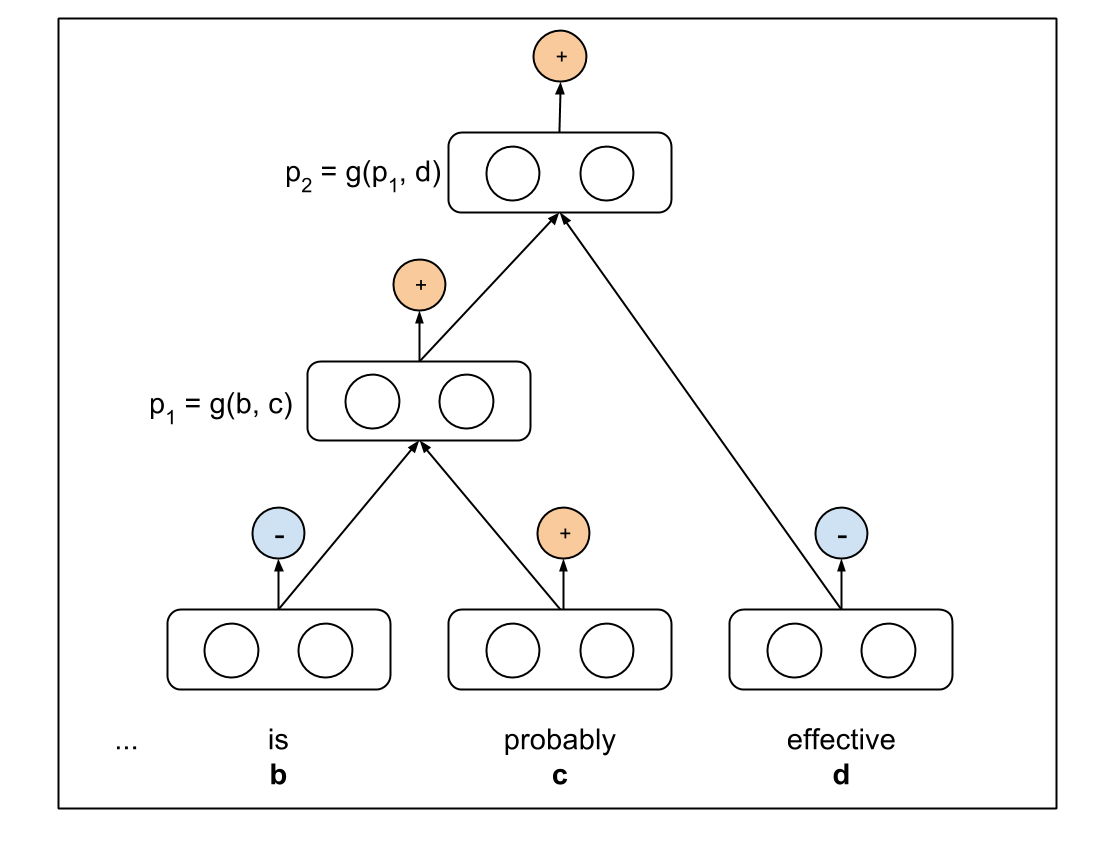
\includegraphics[width=6.5cm,height=8.2cm,keepaspectratio]{rntn1.png}
\caption{Compute parent vectors in a bottom up fashion using a compositionality function g and use node vectors as features for a classifier at that node.\autocite{Socher2013}}
\label{fig:RNTNexpl}
\end{minipage}
\begin{minipage}{.1\textwidth}
\end{minipage}
\begin{minipage}{.45\textwidth}
\centering
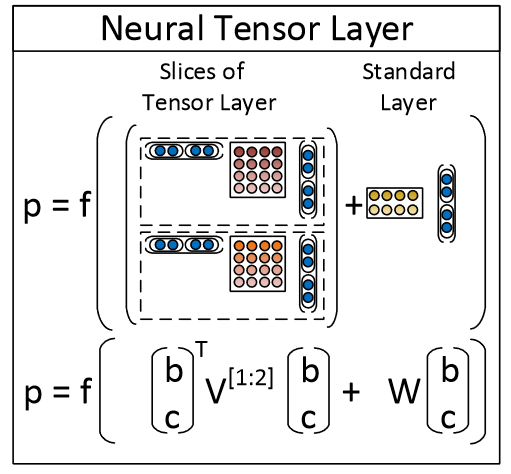
\includegraphics[width=6.6cm,height=7.6cm,keepaspectratio]{neural_tensor_network.PNG}
\caption{A single layer of the Recursive Neural Tensor Network. Each dashed box represents one of {\it d} slices and can capture a type of influence a child can have on its parent \autocite{Socher2013}}
\label{fig:RNTN}
\end{minipage}
\end{figure}

\paragraph{Parse tree generation and labeling} The sentence is first fed into the Stanford parser which tags the Parts-of-Speech (PoS) of the sentence. The nodes of this parse tree are then labeled automatically using the following heuristic: {\it Any node that contains the entire cue phrase is labeled as speculative and all other nodes are labeled as non-speculative}. The labeled parse tree for the example sentence is shown in Figure~\ref{fig:parsetree}. A `$+$' label indicates a speculative node and a `$-$' label indicates a non-speculative node. Such labeled parse trees are obtained for the 14539 sentences taken from the BioScope corpus, which are then split into training/cross-validation/test sets in the proportion 60\%/10\%/30\% respectively.

Training and test sentences are tokenized using the Stanford parser. This is an intelligent word tokenizer which treats brackets, commas and periods as words. By observation, it seems to parse similarly to the NTLK \texttt{ntlk.word\_tokenize} function used in the PV approach.

\paragraph{Training the RNTN} The labeled parse trees are then trained using a RNTN as described in \textcite{Socher2013}. Each word is represented as a $d \times d$ matrix. The parameters of this matrix are trained to minimize the classification error at each node. A tensor based composition function is used for all the nodes as shown in Figure~\ref{fig:RNTN}. In this figure, `b' and `c' are the word vectors of the child nodes (see Figure~\ref{fig:RNTNexpl}) and $V \in \mathbb{R}^{2d \times 2d \times d}$ is the tensor that defines the multiple bilinear forms. The concatenated vector of `b' and `c' is multiplied with each slice $V \in \mathbb{R}^{d \times d}$ and $W \in \mathbb{R}^{d \times 2d}$ is the weight matrix learned. 
% * <rasiga.g@gmail.com> 2014-12-18T15:45:38.146Z:
%
%  add formulae and description
%


In addition to the word matrices, each node has a softmax classifier trained on its vector representation to predict a target vector $t$. The target distribution vector at each node has 0-1 encoding. Since there are two classes for our task, namely {\it speculative} and {\it non-speculative}, $t$ is of length 2 and has a form $[1,0]$ and $[0,1]$ for speculative and non-speculative classes respectively. The KL-divergence between the predicted distribution and the correct distribution is used to maximize the probability of the correct prediction. The backpropagation of error derivatives is done through the structure in the RNTN. The reader is referred to \textcite{Socher2013} for a detailed description of the procedure. 

\paragraph{Testing new sentences} The Stanford parser is used to generate a binary parse tree for each test sentence. The trained RNTN model is then used to predict the speculativeness at each node of the parse tree. The sentence is classified as speculative or not based on the classification of the root node.

\section{Evaluation}

\subsection{Baseline algorithms}

We apply three baseline algorithms to the task of recognizing speculative language in sentences - linear Support Vector Machines (SVM), Naive Bayes (NB) and pattern matching.

\paragraph{Linear SVM, NB} We pre-process sentences the same way with linear SVM and NB. Each sentence is transformed into a Boolean Bag-of-Words (BoW) representation.  Each element in the BOW represents the presence or absence\footnote{Note that we only consider whether a unigram/bigram is present or absent, rather than the number of times the unigram/bigram appears in a sentence. We did try the latter approach on linear SVMs and NB, but it consistently performed worse than the Boolean approach. Hence we leave it out of our report.} of a word, in the case of unigrams, or a pair of words, in the case of bigrams. We train the SVM and NB classifiers with 70\% of the dataset and test them on 30\% of the dataset. No cross-validation is done\footnote{We initially tried to cross-validate the penalty term for the linear SVM but found no significant difference in performance between a wide range of values. This strongly suggests that the bigram BoW representation of the training data is linearly separable.}. We use an SVM penalty term $C$ of 1 and a NB Laplacian smoothing term of 1.

\paragraph{Pattern matching} We use a simple, nonparametric method for pattern matching, in which we identify patterns that are considered speculative from the training data and classify a test sentence as speculative if it contains any of these patterns. The patterns identified as speculative are the phrases annotated as speculative cues in the Bioscope corpus. We use a train-test split of 70\%-30\% as before, with no cross-validation.
% // selection of data (training, testing , validation) \\
% // setting parameters for algos \\
% // what are you trying to test/demonstrate in your experiments - optimize for F1 score on CV set

% describe your experiments and results. Describe your data sets in adequate detail. If you selected a subset of a larger data set, how did you make this selection? Describe how you chose settings for parameters of the algorithms? Clearly state what are you trying to test/demonstrate in your experiments. Your experiments should be motivated by one or more explicitly stated hypotheses or questions.
\subsection{Empirical Evaluation}
\begin{table}
\caption{Performance metrics ranked by F1 score}
\centering
\begin{tabular}{|l c c c c|}
\hline
&&&&\\
\textbf{Method} & \textbf{Accuracy} & \textbf{Precision} & \textbf{Recall} & \textbf{F1 score} \\
\hline
&&&& \\
PV (Bioscope + 1000 BioMed articles) & 0.761 & 0.341 & 0.368 & 0.354 \\
PV (BioScope only) & 0.704 & 0.291 & 0.463 & 0.357 \\
PV (Bioscope + 3000 BioMed articles) & 0.735 & 0.320 & 0.433 & 0.368 \\
Bigram NB & 0.900 & 0.909 & 0.479 & 0.627 \\
Pattern Matching & 0.805 & 0.468 & 0.985 & 0.635 \\
Unigram NB & 0.903 & 0.738 & 0.694 & 0.715 \\
Unigram SVM & 0.957 & 0.911 & 0.835 & 0.871 \\
Bigram SVM & 0.962 & 0.964 & 0.811 & 0.881 \\
RNTN & 0.958 & 0.904 & 0.866 & 0.885 \\
\hline
\end{tabular}
\label{table:F1score}
\end{table}

%The training set for our tasks is 60\% of full\_papers.xml and abstracts.xml taken from the Bioscope corpus. For cross-validation we use 10\% of the corpus and the remaining 30\% is used for testing.


% * <jiashen@gmail.com> 2014-12-18T04:17:31.695Z:
%
%  Need to resolve conflict with what I said about the NLTK parser. We're using two parsers
%
A summary of the results are given in Table~\ref{table:F1score}. Precision-recall curves and ROC curves are shown in Figures~\ref{fig:PR} and \ref{fig:ROC} respectively. Bigram NB and unigram SVM do not perform as well as unigram NB and bigram SVM respectively and are not shown in the figures.

The RNTN has the best F1 score of 0.885, performing marginally better than bigram SVMs (F1 = 0.881). The PV model with no unlabeled data performs the worst (F1 = 0.357), and performance does not improve even after training with 1000 BioMed articles (approx 370K sentences) and 3000 BioMed articles (approx. 1.1 million sentences).


\begin{figure}
\centering
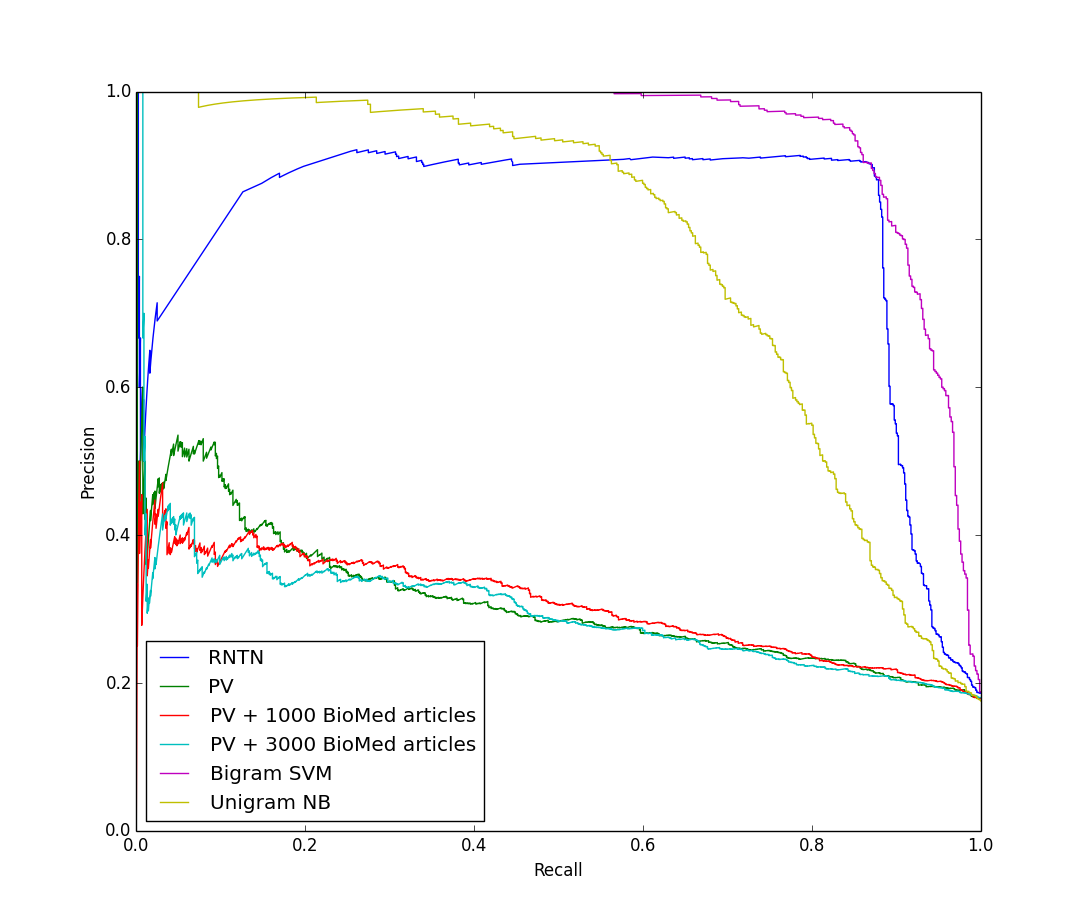
\includegraphics[width=10cm,height=9cm,keepaspectratio]{PR_all.png}
\caption{Precision-recall curves for PV approach, RNTN and baselines.}
\label{fig:PR}
\end{figure}
\begin{figure}
\centering   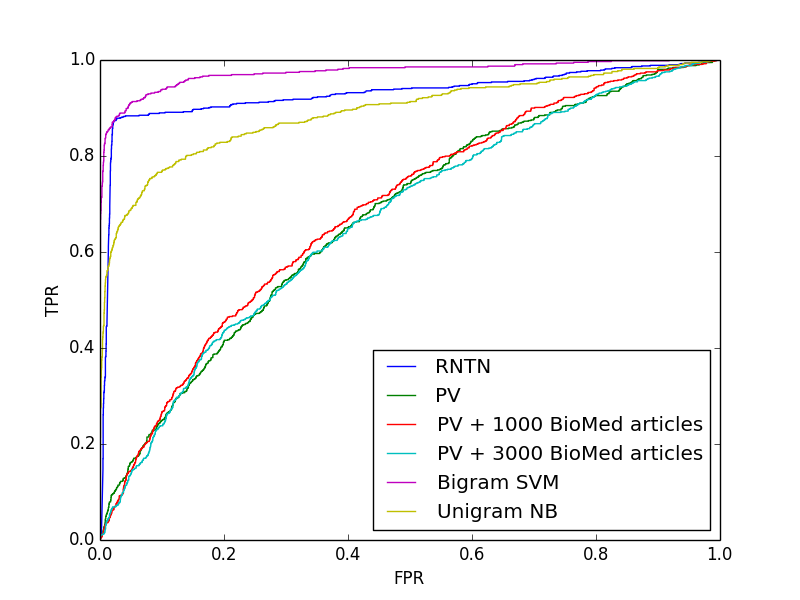
\includegraphics[width=10cm,height=9cm,keepaspectratio]{roc_all.png}
\caption{ROC curves for PV approach, RNTN and baselines}
\label{fig:ROC}
\end{figure}
 
% * <jiashen@gmail.com> 2014-12-18T04:17:18.834Z:
%
%  missing section
%
% ^ <jiashen@gmail.com> 2014-12-18T04:20:13.596Z:
%
%  Need to explain why different algorithms perform differently
%

\section{Discussion}

\paragraph{Baselines} The linear bigram SVM model performs significantly better than both unigram and bigram NB, which suggests that the feature independence assumption of Naive Bayes does not hold true in our data. Due to the nature of pattern matching, the algorithm has very high recall and low precision. High recall occurs because most of the speculative cues that exist in the test set appear in the training set. Low precision occurs because speculative cues may not be speculative depending on their context, e.g., the cue {\it or}. Therefore a speculative cue that appears in a training sentence and appears again in a test sentence may not be speculative in the latter case, resulting in a false postive.

\paragraph{PV approach} There may be several explanations to why the PV approach does poorly. One is that the model failed to converge to a local minimum as the F1 score of the logistic classifier is a poor surrogate for the training accuracy of the PV model. Another is that the training data cannot express the semantic information of its constituent sentences, and therefore a learner cannot learn this information given the data. Intuitively, it would be difficult even for a native English speaker to learn medical biology just by reading biomedical articles, since these articles assume an expert level of knowledge in the field. A similar scenario may be occurring in this unsupervised training algorithm. For this reason, it may prove useful to train the model initially with easier text such as college-level textbooks before fine-tuning the model with academic articles. Yet another possible explanation is that the model has overfit the training data, and should be trained with more data. Note that we only used about 1\% of the articles in the BioMed corpus in this study.


\paragraph{RNTN} The RNTN approach produces much better results than the Paragraph Vector Representation, suggesting that speculative language recognition is amenable to formulation as a sentiment analysis task using RNTN.

The ROC and precision-recall curves for RNTN have a more angular structure than the other methods. This is because the confidence value for a sentence identified as speculative is very close to 1, causing sharp angles in the beginning and the ends of the ROC and precision-recall curves respectively. In other words, when the classifier identifies a sentence as speculative, it does so with high confidence,  regardless of correctness.

While RNTN produces the best F1 score in our experiments, its performance is just marginally better than our best performing baseline, linear bigram SVMs. The comparable success of linear SVMs indicates that  speculative language recognition may be reasonably approximated as a classification task for linearly separable data, and may not benefit significantly from more sophisticated approaches using distributed word representations. Additionally, one disadvantage of RNTN is that its training is significantly slower than the other methods.

\subsection*{Limitations of our approach} 
The features used by our methods do not include meta-information such as author and affiliations, which may have a prior on propensity for speculative language. This information if available, can be used for validating the reliability of the information in a biomedical article. Also, each sentence is considered as an independent sentence and does not consider neighboring sentences or paragraphs. Furthermore, in our implementations, we have considered the absence of a speculative cue word/phrase as indicative of a non-speculative sentence. But there are cases when a sentence without a speculative cue word has some speculation. For instance, consider an assertion relating to a result that does not necessarily follow from work presented, but could be extrapolated from it \autocite{Light2004}. Even though this assertion might not include speculative cue words, it should not be regarded as an established fact.

A technical limitation of the PV approach is that it stores the paragraph vectors of all training sentences. Therefore its memory complexity is linear in the number of training sentences, compared to RNTN which is linear in the size of the vocabulary but approximately constant in the number of training sentences. Of the two, RNTN scales better with larger amounts of training data. However, RNTN is trained only on labeled data, so it cannot exploit the large set of unlabeled biomedical articles.
% * <rasiga.g@gmail.com> 2014-12-18T02:20:19.238Z:
%
%  add limitation of the PV's API
%
% ^ <jiashen@gmail.com> 2014-12-18T04:47:15.042Z.

\section{Conclusion}

We investigate the application of the distributed representation of sentences to the task of speculative language recognition in biomedical text. We try two methods that transform a test sentence into a distributed representation, RNTN and the PV approach, and compare these two methods against several simple baseline algorithms. We find some evidence to support our hypothesis that this representation improves performance in the recognition task. The RNTN performs slightly better than linear bigram SVM, our best-performing baseline algorithm, but we also note that the marginal improvement of 0.4\% in F1 score is at the cost of high computational time. The PV approach performs significantly worse than all other algorithms in this study, even when the PV learner is trained with a large unlabeled dataset. 

The PV approach has the potential to learn high-quality distributed representations of sentences by exploiting a large unlabeled dataset. It is the only algorithm in this study that can be unsupervised. However, how to tune the parameters used at test time is an open problem. Future research may include investigating this problem, or pretraining the model with general text such as Wikipedia articles. In addition to classifying sentences, we may also investigate determining the scope of the speculative cue words in speculative sentences.

\printbibliography{}

\pagebreak
\begin{center}
\section*{Appendix}
\end{center}

\section*{How to evaluate the PV model}

One drawback of an unsupervised learning method such as the Paragraph Vector model is the difficulty in evaluating the learned model. In this study, we considered two evaluation methods that evaluated only the learned word vectors, based on Google's word relationship set\footnote{\url{https://code.google.com/p/word2vec/}} \autocite{mikolov2013efficient}. Each relationship is a 4-tuple that can be categorized as a semantic relationship (e.g., Italy is to Rome as France is to Paris) or a syntactic relationship (e.g. run is to running as grow is to growing). With this 4-tuple and word-to-vector mapping, we can try to predict one of the words in the 4-tuple given the other three words, e.g., try to answer `Paris' given the question `{\it Italy} is to {\it Rome} as {\it France} is to {\it ?}'.

One possible evaluation metric would be the accuracy of a prediction task, in which a model is considered correct if the true label (e.g., Paris) is in one of the model's top 5 predictions.  Another possible metric is the average distance between the two deltas of the 4-tuple, e.g. we measure the distance between $vec(Italy) - vec(Rome)$ and $vec(France) - vec(Paris)$, where $vec$ is a function that maps a word to its vector.  A good model should give a small distance between these two terms. The metric is the average distance of the set of 4-tuples.

To this end, a better word relationship evaluation set should be developed specific to biomedical language. In Google's relationship set, much of the vocabulary in the semantic relationships is absent in biomedical language. For example, you will be hard-pressed to find the names of countries and capitals in biomedical articles. Hence, a large portion of the relationship set has to be excluded if used on a biomedical dataset. We suggest creating a set of semantic relationships for biomedical language (e.g., headache is to aspirin as cough is to dextromethorphan). While these may not be as unequivocal as country-capital relationships, they serve as a quick way to evaluate word vectors.

\end{document}


